\documentclass[UTF8]{ctexart}
\usepackage{graphicx}
\usepackage{amsmath}
\usepackage{cite}
\usepackage{mathtools}
\usepackage[a4paper,left=2.5cm,right=2.5cm,top=3cm,bottom=3cm]{geometry}
\title{声速的测量:实验报告}
\author{禤科材 PB20030874 20级14系 707组 1号台}
\date{\today}
\bibliographystyle{plain}
\begin{document}
    \maketitle

   \section{实验目的}

   \begin{center}
    1.测量压电陶瓷换能器的谐振频率

    2.用驻波法和相位比较法测量气体、液体中的声速

    3.用时差法测量固体中的声速 
   \end{center}

    \section{实验原理}

    \begin{center}
        \emph{\zihao{-4}声波在空气中的传播速度}\\[0.4cm]
    \end{center}

    声波在理想气体中的传播速度为:
    \begin{equation}
        \nu =\sqrt{\frac{\gamma RT}{M}}
    \end{equation}

    式中$\gamma $是气体的定压比热容和定容比热容之比,R是普适气体常量,M 是气体的摩尔
    质量,T 是热力学温度。由式(1)可见,气体的温度和性质是影响空气中声速的主要因素。如果
    忽略空气中的水蒸气和其他夹杂物的影响,在标准状态下干燥的理想空气中的声速为:
    \begin{equation*}
        \nu =\sqrt{\frac{\gamma RT_0}{M}}=331.45(m·s^{-1})
    \end{equation*}

    若同时考虑温度和空气中水蒸气的影响,校准后声速公式为:
    \begin{equation}
        \nu =331.45\sqrt{(1+\frac{t}{273.15}))(1+\frac{0.3192p_w}{p})}(m·s^{-1})
    \end{equation}
    式中$p_w$为水蒸气的分压强,$p$ 为大气压强。而 $p_w=p_sH$,其中 $p_s$为测量温度下空气中水蒸气的饱
    和蒸气压(可以从饱和蒸气压和温度的关系表中查出),$H$ 为相对湿度,可以从干湿度温度计上读出。

    \begin{center}
        \emph{\zihao{-4}声速测量的实验方法}\\[0.4cm]
    \end{center}

    根据波动理论,在介质中传播的声波,波速、波长和频率之间的关系为:
    \begin{equation}
        \nu =\lambda *f
    \end{equation}
    在实验中,可以通过测定声波的波长和频率求声速。声波的频率$f$等于声源的电激励信
    号频率,该频率可由数字频率计测出,或由低频信号发生器上的频率直接给出,而声波的波长$\lambda $
    则常用共振干涉法(驻波假设下)和相位比较法(行波近似下)来测量。

    \emph{1.共振干涉法}

    

    实验装置原理如图,S1、S2 为压电换能器,S1 为声波发射源,S2 为声波接收器,当 S2 的
    接收表面直径较大时,将会反射部分和声源同频率的声波。入射波和反射波振动方向与频率相同
    而发生相干叠加,形成“驻波”,声场中将会形成稳定的强度分布,在示波器上观察到的是这两个相干波在 S2 处合成振动的情况。

    \begin{figure}[ht]
        \centering 
        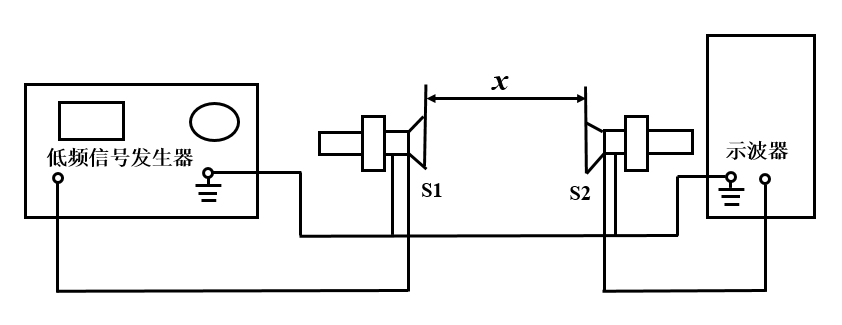
\includegraphics[width=8cm]{驻波法.png}
    \end{figure}

    根据声学理论,在声场中空气质点位移为波腹的地方,声压最小;而空气质点位移为波节的地方,声压
   最大。由纵波的性质可以证明,当发生共振时,接收器 S2 反射端面位置近似为振幅的“波节”,此处位移为 0,接收到的声压信号最强。连续改变距离 L,示波器
   可观察到,声压波幅将在最大值和最小值之间呈周期性变化。
   
   所以当 S1、S2 之间的距离变化量 $\varDelta l$ 为半波长 $\lambda /2$ 的整数倍 n 时,出现稳定的驻波共振现象,声压最大,
   相邻两次声压波幅极大值所对应的距离的变化即为半波长。


    \emph{2.相位比较法}

    实际上,在发射器和接收器间存在的是驻波与行波的叠加。由于
    接收器的反射面不是理想的刚性平面,它对入射声波能量的吸收作用以及空气对声波的吸收作用促使声波
    振幅将随传播距离而衰减。所以,还可以通过比较声源处的声压的相位来测定声速。这称为相位比较法或行波法。

    \begin{figure}[ht]
        \centering 
        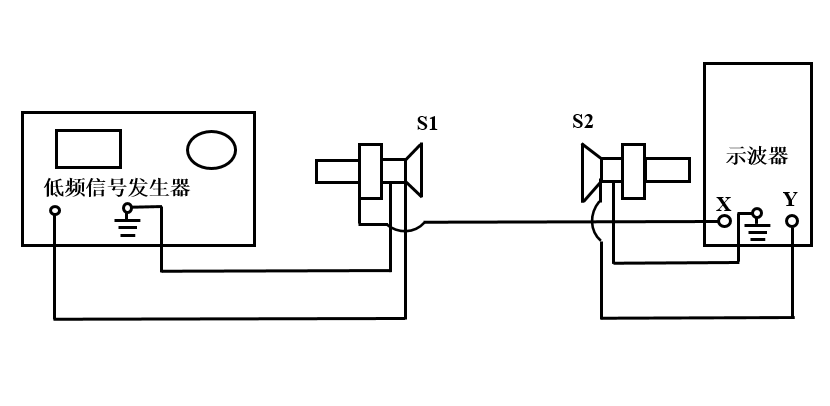
\includegraphics[width=8cm]{相位法.png}
    \end{figure}

    发射器与接收器之间有相位差,可通过李萨如图形来观察。随着振动的相位差从 $0-\pi $ 的变化,李萨如图形从斜率为正
    的直线变为椭圆,再变到斜率为负的直线。因此,每移动半个波长,就会重复出现斜率符号相反的直线。
    
    \emph{3.时差法(脉冲法)}

    以上两种方法测量声速,是用示波器观察波峰和波谷,或者观察两个波的相位差,原理是正
确的,但是读数位置不易确定。较精确测量声速是用声波时差法。它是将脉冲调制的电信号加到发射换能器上,声波在媒质中传播,从信号源经过时间 t 后,
到达距离为 L 处的接收换能器,那么可以用以下公式求出声波在媒质中传播的速度:
\begin{equation}
    \nu =\frac{L}{t}
\end{equation}


    \section{实验设备}

     SV5 型声速测量仪(含水槽)
     
     双踪示波器

     非金属(有机玻璃棒)

    金属(黄铜棒)

    游标卡尺

    \section{实验步骤}

    \begin{center}
        \emph{\zihao{-4}共振干涉法测量空气中的声波波长与声速}\\[0.4cm]
    \end{center}
    
    \emph{测量谐振频率}

    在 S1 和 S2 之间保持一定间距的情况下,观察接收波的电压幅度变化,调节正弦信号频率,
    当在某一频率点处电压幅度最大时,此频率即为压电换能器 S1、S2 的相匹配频率点,即为谐振频率 f。

    \emph{开始测量}

    当 S1 和 S2 相距 5 cm 以上时,转动鼓轮移动 S2,观察波的干涉现象,当示波器上出现振幅
   最大信号时,记下 S2 的位置 L0。由近而远或由远而近改变接收器 S2 的位置,均可以观察到正
   弦波形发生周期性的变化,逐个记下振幅最大的波腹的位置共 12 个位置点。并用最小二乘法处理
   数据,计算波长和声速及其不确定度。

    \begin{center}
        \emph{\zihao{-4}相位比较法测量水中的波长和声速}\\[0.4cm]
    \end{center} 
    
    在储液槽中装入水至刻度线,将换能器置于储液槽中,正确接线。令示波器置于“X-Y”垂直振动合成模式,此时可
    以看到示波器上出现椭圆或斜直线的李萨如图形。当 S1 和 S2 相距 5 cm 以上时,转动鼓轮移动
    S2,观察图形,依次测出李萨如图形斜率正、负变化的直线出现时 S2 的位置 Li,共记录 8 个位置值。用作图法处理数据,计算水中的波长和声速。

    \begin{center}
        \emph{\zihao{-4}设计实验——用时差法测量有机玻璃棒和黄铜棒中的声速}\\[0.4cm]
    \end{center}

    正确接线,将专用信号源上的“测试方法”调至“脉冲波”的位置,“声速传播媒质”按测试材质的不同,调至“非金属”或“金属”的位置。

    分别测量三种不同长度的有机玻璃棒和黄铜棒,记录下录信号源的时间读数,此时显示的时间为从信号源发出脉冲信号到接收端接
    收所用的时间。测试棒的长度可用游标卡尺测量得到并记录长度 L。

    使用作图法处理实验数据,计算出介质中的声速。

    \section{实验记录}
    实验数据附于报告最后

    \section{数据处理}

    \begin{center}
        \emph{\zihao{-4}共振干涉法}\\[0.4cm]
    \end{center}
    
    以声压波幅极大值出现的先后序号为X轴、$L_1$和$L_2$间隔距离为Y轴,作图,斜率即是空气中声波的半波长:

    \begin{figure}[ht]
        \centering 
        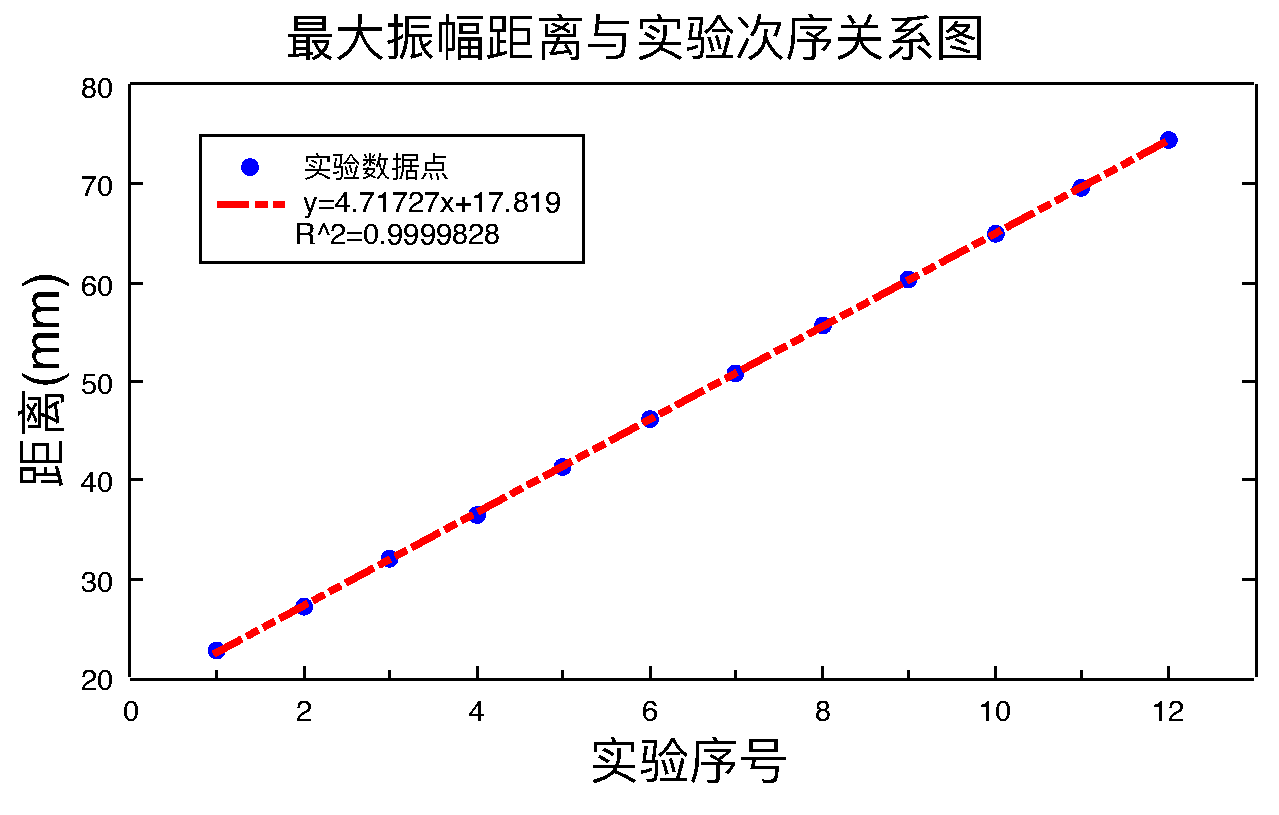
\includegraphics[width=15cm]{共振干涉.pdf}
    \end{figure}

    从图中可以看出,实验数据点基本分布在拟合直线左右,且相关系数$R^2$高达0.9999828,表明实验数据相关性很强,可信度高。

    \emph{斜率$k$的标准差:}
    \begin{equation*}
        \sigma_k =k\sqrt{(\frac{1}{R^2}-1)/(n-2)}=4.71727\sqrt{(\frac{1}{0.9999828}-1)/(12-2)} =0.0061866(mm)
    \end{equation*}

    \emph{斜率$k$展伸不确定度:}
    \begin{equation*}
        U_{0.95}=t_p·\sigma_k=2.23·0.0061866=0.0137963(mm)
    \end{equation*}

    \emph{截距$b$标准差:}
    \begin{equation*}
        \sigma_b=\sqrt{\overline{{x^2}}}·\sigma_k=\sqrt{\frac{1^2+2^2+3^2+4^2+5^2+6^2+7^2+8^2+9^2+10^2+11^2+12^2}{12}}*0.0061866=0.045532
    \end{equation*}

    \emph{截距$b$展伸不确定度:}
    \begin{equation*}
        U_{0.95}=t_{0.95}·\sigma_b=2.23*0.045532=0.1015382
    \end{equation*}
    
    根据波速、波长、频率计算公式计算得到:
    \begin{equation*}
        v=37062*4.71727*2/1000=349.663(m/s)
    \end{equation*}

    根据不确定度合成公式:
    \begin{equation}
        (\frac{U_v}{v})^2=(\frac{U_k}{k})^2+(\frac{U_f}{f})^2
    \end{equation}

    将频率不确定度记为0,计算得到:
    \begin{equation*}
        U_v=v*\sqrt{(\frac{U_k}{k})^2+(\frac{U_f}{f})^2}=349.663*\sqrt{(\frac{0.0137693}{4.71727})^2+(\frac{0}{37062})^2}=1.021(m/s)
    \end{equation*}

    \emph{\zihao{-4}最终结果:}
    \begin{equation}
        v=349.663±1.021(m/s)
    \end{equation}


    根据校准后的声速公式(2),计算当前温度下的理论声速:
    \begin{equation*}
        v=331.45\sqrt{(1+\frac{25.4}{273.15})*(1+\frac{0.3192*3167.68*0.50}{101325})}=347.381(m/s)
    \end{equation*}

    相对误差:
    \begin{equation*}
        \varphi =\frac{349.663-347.381}{347.381}=6.6*10^{-3}
    \end{equation*}

    从数据中可知,误差在实验设计允许的范围内。


    \begin{center}
        \emph{\zihao{-4}相位比较法}
    \end{center}

    以李萨茹图形出现斜率符号相反的直线的次序为X轴、对应的距离为Y轴,直线斜率即是声波的半波长:

    \begin{figure}[ht]
        \centering 
        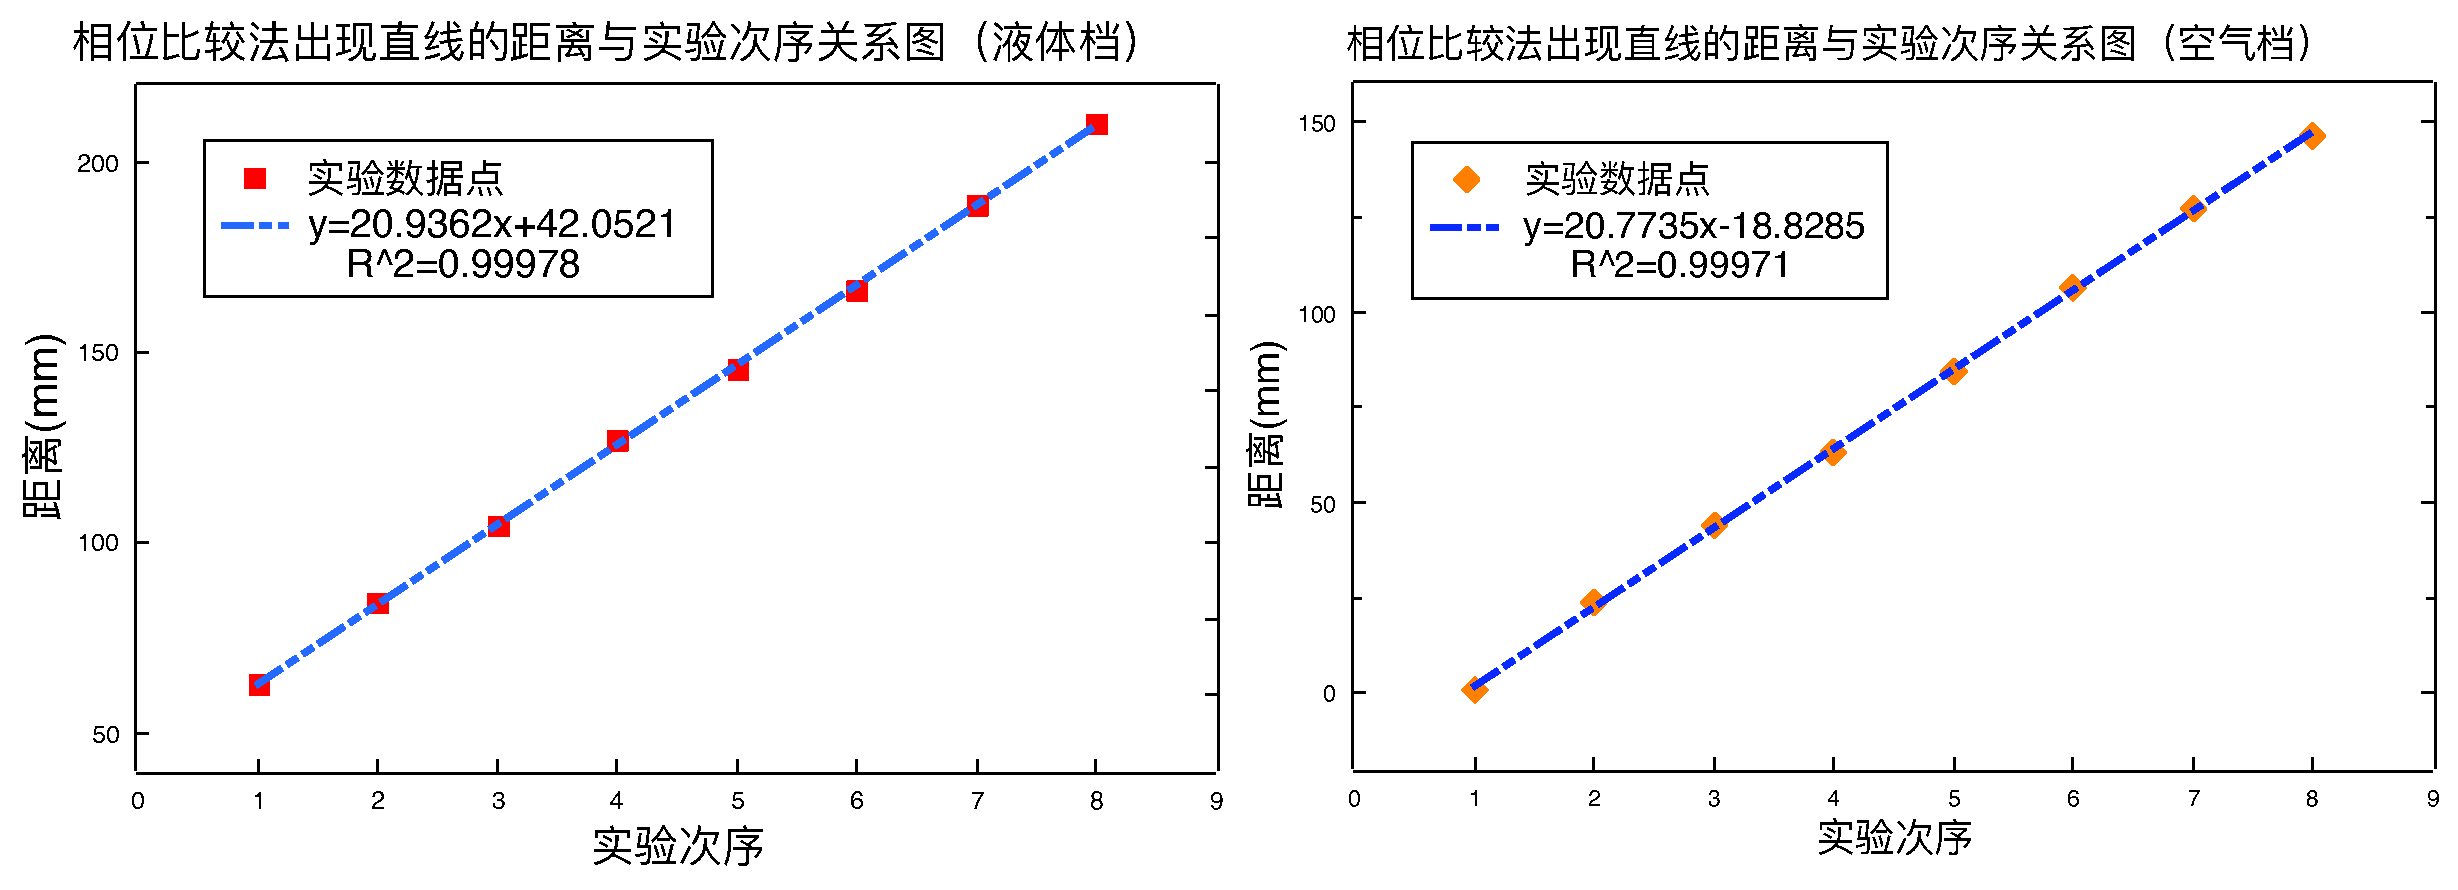
\includegraphics[width=17cm]{相位比较.pdf}
    \end{figure}

    从图中可以看出,实验数据点基本分布在拟合直线左右,且相关系数较大,表明实验数据线性相关程度较高,实验数据可信度较大。分别使用液体档位和空气档位计算声速如下:

    \begin{equation*}
        v_{liquid/option}=37062*20.9362*2/1000=1551.874(m/s)
    \end{equation*}

    \begin{equation*}
        v_{air/option}=37062*20.7735*2/1000=1539.814(m/s)
    \end{equation*}


    \begin{center}
        \emph{\zihao{-4}脉冲法}\\[0.4cm]
    \end{center}

    以时间为X轴、棒长度为Y轴作图,拟合直线斜率即是声速在对应介质中的值:

    \begin{figure}[ht]
        \centering 
        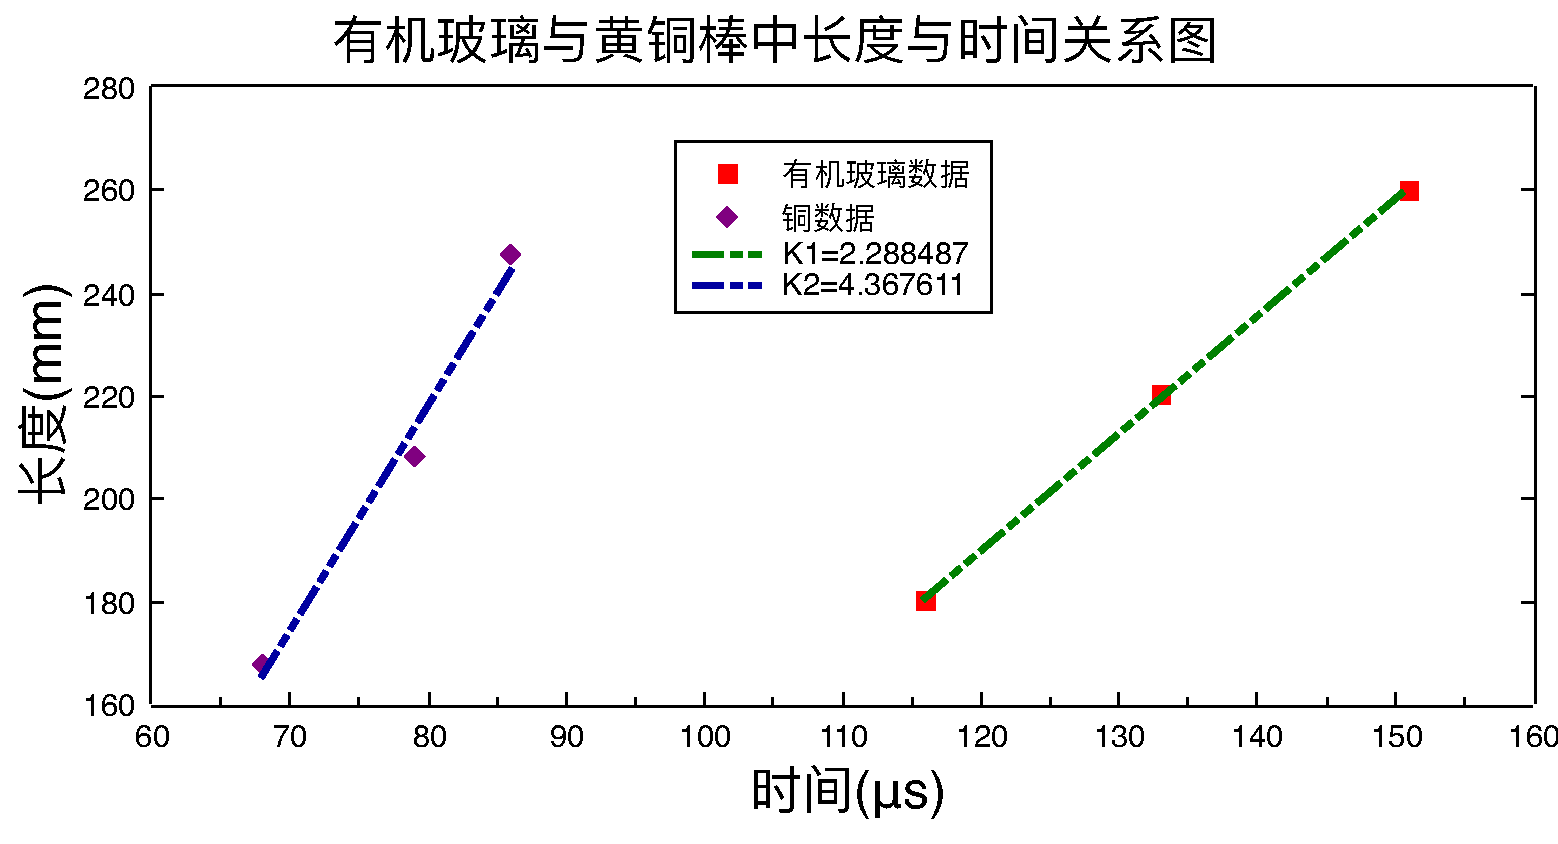
\includegraphics[width=15cm]{设计实验.pdf}
    \end{figure}

    计算可得有机玻璃和黄铜中的声速如下:

    \begin{equation*}
        v_{PMMA}=2288.487(m/s)
    \end{equation*}

    \begin{equation*}
        v_{copper}=4367.661(m/s)
    \end{equation*}

    \section{误差分析}

    \emph{水中声速的测量}
    
    查询资料得知,在20度下的纯水中声速为1482.9m/s,此后每温度升高一度,声速大概升高4.6m/s。
    在实验条件25.4度下,计算可知声速应当是1507m/s,与实验测量值1551.874m/s相差较大,原因分析如下:

    第一,实验用水不是纯净水,而是含有一些杂质离子的自来水,振动能量可能在这些杂质周围传递较快,导致了测量值偏大的结果。

    第二,实验时水不是完全静止的,在调节压电能量转换器时有所震荡,其中沿声波振动方向传递的水波会导致测量值偏大。

    第三,由于声波能量在传递过程中会衰减,以致李萨茹图形中小短轴椭圆和直线随着实验的进行区别减小,导致实验人判断李萨茹图形是否是直线时有所延迟,波长偏大,测量值偏大。

    此外,观察到使用空气档位和使用液体档位测量得到的声速差别较大。为什么相同的振动频率,在不同档位下测量到的声速不同?由于空气密度比水的密度小,
    可能是因为在液体档位下,实验仪器更灵敏,一些较为轻微的振动也计入,而空气档位下实验仪器较为迟钝,测量到的声速偏小。

    \emph{黄铜棒中声速的测量}

    作出图像后观察到黄铜的实验数据点和拟合曲线偏差较大,可能是因为测量时未能将接口润滑剂涂抹均匀,也可能没有旋紧插头就读数。


    \section{思考题}
    
    \emph{\\[0.02cm]\zihao{-4}1.定性分析共振法测量时,声压振幅极大值随距离变长而减小的原因?}

    声波在传递过程中,能量不可避免的衰减导致振幅有所降低。

    \emph{\\[0.2cm]\zihao{-4}2.声速测量中驻波法、相位法、时差法有何异同?}

    共振干涉法和相位比较法:都是利用声速与频率、波长的关系来测量声速,且给定频率。但共振法假设驻波干涉,通过两次振幅极值的位移差来获得波长值;
    相位比较法是通过比较波源与接收波的相位差来获得波长值。

    脉冲法:时差法与以上两种方法不同,它不依赖于声波的形式,通过直接测量声波通过一段已知长度的介质所需的时间来计算声速,所以使用的是脉冲波。

    \emph{\\[0.2cm]\zihao{-4}3.各种气体中的声速是否相同,为什么?}

    不同。首先,如果温度不同,显然会对气体中的声速造成影响;齐次,由声速公式(1)可知,
    如果T相同、R相同,依然有定压比热容和定容比热容之比$\gamma $和摩尔质量$M$两个参数影响声速大小,而这两个参数
    由气体的固有性质决定。
    
    \nocite{dawushiyan}
    \nocite{shiyanjiaocheng}
    \nocite{jiangyi}
    \bibliography{math}

\end{document}
